\documentclass{beamer}
\usetheme{CambridgeUS}
\usecolortheme{default}
\usepackage[utf8]{inputenc}
\usepackage{lmodern}
\usepackage{graphicx}
\usepackage{hyperref}
\usepackage{tikz}
\usepackage{pgfplots}
\usetikzlibrary{3d, positioning, arrows.meta}


\title{Research Critique of AlphaPeptDeep}  
\subtitle{Modular Deep Learning Framework for Proteomics} 
\author{Vignesh Babu J S and Saranath P}
\date{\today}

\begin{document}

% Title Slide
\begin{frame}
  \titlepage
\end{frame}

% Outline Slide
\begin{frame}
  \frametitle{Outline}
  \tableofcontents
\end{frame}

\section{Motivation and Story}
\begin{frame}
  \frametitle{Motivation and Story}
  \begin{columns}
    \column{0.55\linewidth}
      \begin{itemize}
        \item Imagine navigating a sprawling, ancient city where every street holds clues to a rich history.
        \item In proteomics, each peptide is like a unique building—some with subtle renovations (post-translational modifications) or built by unconventional architects (non-tryptic peptides).
        \item Traditional identification methods often struggle to map this intricate cityscape, leading to misidentification in complex samples.
      \end{itemize}
    \column{0.45\linewidth}
      % Replace 'ancient_city.jpg' and 'peptide_structure.jpg' with your actual image file names
      \includegraphics[width=0.7\linewidth]{image1.jpeg}\\[1em]
      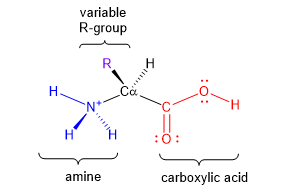
\includegraphics[width=0.7\linewidth]{peptide.png}
  \end{columns}
\end{frame}

\begin{frame}
  \frametitle{Mapping the Proteomics Landscape}
  \begin{itemize}
    \item Accurate prediction of peptide properties provides the precise map needed to align experimental spectra with theoretical models.
    \item \textbf{Retention Time Prediction:} Establishes when peptides elute during Liquid Chromatography–Mass Spectrometry runs.
    \item \textbf{Mass Spectrometry Stage 2 (MS2) Prediction:} MS2 is the second stage of mass spectrometry where peptides are fragmented to produce ion spectra; the prediction forecasts the intensities of these fragment ions for matching observed spectra.
    \item \textbf{Collision Cross-Section Prediction:} Offers insight into peptide shape and size via ion mobility.
    \item Together, these predictions enhance peptide identification accuracy in complex samples.
  \end{itemize}
\end{frame}

\section{Biological Question and Impact}
\begin{frame}
  \frametitle{Biological Question and Impact}
  \begin{block}{Biological Question}
    How can we improve the accuracy of peptide identification in mass spectrometry-based proteomics?
  \end{block}
  \begin{itemize}
    \item Decoding even the most modified peptides enhances our understanding of complex biological systems.
    \item Improved accuracy paves the way for breakthroughs in disease diagnostics and personalized medicine.
  \end{itemize}
\end{frame}

\section{Computational Problem}
\begin{frame}
  \frametitle{Computational Problem}
  \begin{itemize}
    \item \textbf{Problem:} Develop models that predict peptide properties from amino acid sequences.
    \item \textbf{Nature of the Problem:} A combined regression and classification task where modular architectures and transfer learning help manage variability in experimental conditions.
  \end{itemize}
\end{frame}

\begin{frame}
  \frametitle{Key Algorithms and Computational Methods}
  \begin{itemize}
    \item \textbf{Modular Framework:} Built on PyTorch, featuring a “model shop” for rapid development.
    \item \textbf{Neural Architectures:} Uses LSTM, Transformer, and CNN layers.
    \item \textbf{Transfer Learning:} Adapts pre-trained models to specific conditions with minimal data.
    \item \textbf{Advanced Embedding:} Transforms amino acid sequences and PTMs into numeric tensors.
  \end{itemize}
\end{frame}

\section{Research Critique}
\begin{frame}
  \frametitle{Biological Motivation and Challenge}
  \begin{itemize}
    \item \textbf{Use Case:} Enhance peptide identification sensitivity and specificity by matching predicted properties to experimental MS data.
    \item \textbf{Challenge:} Addressing variability due to diverse PTMs, non-tryptic peptides, and different LC conditions while retaining a flexible and extensible framework.
  \end{itemize}
\end{frame}

\begin{frame}
  \frametitle{What should we predict? }
  \begin{itemize}
    \item \textbf{MS2 Prediction:}
      \begin{itemize}
        \item \textbf{What is MS2?} The second stage of mass spectrometry, where peptides are fragmented to generate ion spectra.
        \item \textbf{Purpose:} Predict the intensities of these fragment ions from a given peptide sequence.
        \item \textbf{Application:} Helps match theoretical spectra to experimental data for accurate peptide identification.
      \end{itemize}
    \item \textbf{RT Prediction:}
      \begin{itemize}
        \item \textbf{What is RT?} Retention Time—the time a peptide takes to elute from the chromatography column.
        \item \textbf{Purpose:} Estimate when each peptide will appear in the LC-MS run.
        \item \textbf{Application:} Enhances alignment of peptide signals and improves identification confidence.
      \end{itemize}
  \end{itemize}
\end{frame}

\begin{frame}
  \frametitle{What should we predict? - contd.}
  \begin{itemize}
    \item \textbf{CCS Prediction:}
      \begin{itemize}
        \item \textbf{What is CCS?} Collision Cross Section—a measure of the peptide's shape and size as it travels through a gas.
        \item \textbf{Purpose:} Predict the ion mobility properties of peptides.
        \item \textbf{Application:} Refines peptide identification by correlating predicted and measured CCS values.
      \end{itemize}
    \item \textbf{PTM Transfer Learning:}
      \begin{itemize}
        \item \textbf{What are PTMs?} Post-Translational Modifications—chemical changes that occur on peptides after translation (e.g., phosphorylation).
        \item \textbf{Purpose:} Adapt pre-trained models to accurately predict the impact of PTMs on MS2, RT, and CCS.
        \item \textbf{Application:} Improves predictions for modified peptides using limited additional data.
      \end{itemize}
  \end{itemize}
\end{frame}

\section{Proposed Approach}
\begin{frame}
  \frametitle{Traditional vs. Proposed Approach}
  \begin{itemize}
    \item \textbf{Traditional Methods:} Use simpler regression models or rule-based approaches (e.g., iRT-calculators, RTPredict, ELUDE).
    \item \textbf{Proposed Approach:} AlphaPeptDeep employs deep learning models (LSTM, Transformer, CNN) with a modular design and transfer learning capabilities.
    \item \textbf{Key Difference:} Modularity via the “model shop” enables easy extension and rapid prototyping, adapting to new experimental setups.
  \end{itemize}
\end{frame}

\section{Architecture}
\begin{frame}
  \frametitle{MS2 Model Architecture (Part 1)}
  \begin{itemize}
    \item \textbf{Input \& Embedding:}
      \begin{itemize}
        \item Input: Peptide sequence, PTMs, and metadata (e.g. charge, collisional energy, instrument type).
        \item Embedding layer converts these inputs into numerical tensors.
      \end{itemize}
    \item \textbf{Positional Encoding:}
      \begin{itemize}
        \item Adds sequence position information to the embedded tokens.
      \end{itemize}
    \item \textbf{Transformer Layers:}
      \begin{itemize}
        \item Four transformer layers (hidden size = 256) to capture complex sequence dependencies.
      \end{itemize}
  \end{itemize}
\end{frame}

\begin{frame}
  \frametitle{MS2 Model Architecture (Part 2)}
  \begin{itemize}
    \item \textbf{Additional Transformer:}
      \begin{itemize}
        \item Extra transformer layer predicts \textit{mod-loss} (e.g., -98 Da loss for phospho).
        \item Can be disabled via \texttt{mask\_modloss=True}.
      \end{itemize}
    \item \textbf{Output Layer:}
      \begin{itemize}
        \item Two fully-connected (FC) layers output a tensor of dimensions $(n-1) \times 8$, where $n$ is the peptide length.
        \item Eight channels represent fragment ion types: \texttt{b\_+}, \texttt{b\_++}, \texttt{y\_+}, \texttt{y\_++}, \texttt{b\_modloss\_+}, \texttt{b\_modloss\_++}, \texttt{y\_modloss\_+}, and \texttt{y\_modloss\_++}.
      \end{itemize}
    \item \textbf{Training Details:}
      \begin{itemize}
        \item \textit{Phase 1 (Tryptic peptides):} Epoch=100, warmup=20, lr=$1e^{-5}$, dropout=0.1.
        \item \textit{Phase 2 (HLA peptides):} Epoch=20, warmup=5, mini-batch size=256.
        \item \textit{Phase 3 (Phosphorylation/Ubiquitylation):} Epoch=20, warmup=5, using only PTMs with >0.75 localization.
        \item Total parameters: $\sim3.99$ million.
      \end{itemize}
  \end{itemize}
\end{frame}

\begin{frame}
  \frametitle{RT Model Architecture (Part 1)}
  \begin{itemize}
    \item \textbf{Input \& Embedding:}
      \begin{itemize}
        \item Converts peptide sequences and PTMs into embedded vectors.
      \end{itemize}
    \item \textbf{Convolutional Layer:}
      \begin{itemize}
        \item A CNN layer extracts local sequential features.
      \end{itemize}
    \item \textbf{Recurrent Layers:}
      \begin{itemize}
        \item Two LSTM layers (hidden size = 128) capture long-range dependencies.
        \item Outputs from the last LSTM are summed over the sequence length.
      \end{itemize}
  \end{itemize}
\end{frame}

\begin{frame}
  \frametitle{RT Model Architecture (Part 2)}
  \begin{itemize}
    \item \textbf{Fully-Connected Layers:}
      \begin{itemize}
        \item Two FC layers with output sizes 64 and 1 produce the final RT prediction.
      \end{itemize}
    \item \textbf{Training and Normalization:}
      \begin{itemize}
        \item Total parameters: 708,224.
        \item RT values normalized by LC gradient length (range: 0 to 1).
        \item Training: Epochs = 300, warmup epochs = 30, lr = $1e^{-4}$, dropout = 0.1, mini-batch size = 256.
        \item Fine-tuning: Epochs = 30, warmup = 10.
      \end{itemize}
    \item \textbf{Conversion:}
      \begin{itemize}
        \item For evaluation, predicted RTs are rescaled by the gradient length.
        \item A linear model built on 11 peptides with known iRT values converts predictions to iRT space.
      \end{itemize}
  \end{itemize}
\end{frame}

\begin{frame}
  \frametitle{CCS Model Architecture (Part 1)}
  \begin{itemize}
    \item \textbf{Input \& Embedding:}
      \begin{itemize}
        \item Encodes peptide sequences, PTMs, and precursor charge states.
      \end{itemize}
    \item \textbf{Convolutional Layer:}
      \begin{itemize}
        \item A CNN layer extracts local features from the embedded sequence.
      \end{itemize}
    \item \textbf{Recurrent Layers:}
      \begin{itemize}
        \item Two LSTM layers (hidden size = 128) capture sequential dependencies.
        \item Outputs are summed across the peptide length dimension.
      \end{itemize}
  \end{itemize}
\end{frame}

\begin{frame}
  \frametitle{CCS Model Architecture (Part 2)}
  \begin{itemize}
    \item \textbf{Fully-Connected Layers:}
      \begin{itemize}
        \item Two FC layers with sizes 64 and 1 output the scalar CCS value.
      \end{itemize}
    \item \textbf{Training Details:}
      \begin{itemize}
        \item Total parameters: 713,452.
        \item Training parameters: Epochs = 300, warmup epochs = 30, lr = $1e^{-4}$, dropout = 0.1, mini-batch size = 256 (L1 loss).
      \end{itemize}
    \item \textbf{Conversion:}
      \begin{itemize}
        \item Predicted CCS values are converted to ion mobilities for Bruker timsTOF using the Mason–Schamp equation.
      \end{itemize}
  \end{itemize}
\end{frame}

\begin{frame}{Architecture Diagram}
 \begin{center}
    \includegraphics[width=\textwidth]{Screenshot from 2025-03-12 20-33-16.png}
  \end{center}
    
\end{frame}
\begin{frame}
  \frametitle{HLA: Background and Importance}
  \begin{itemize}
    \item \textbf{What is HLA?}
      \begin{itemize}
        \item HLA stands for \textbf{Human Leukocyte Antigen}.
        \item These are protein fragments (peptides) presented on the cell surface by major histocompatibility complex (MHC) class I molecules.
      \end{itemize}
    \item \textbf{Biological Role:}
      \begin{itemize}
        \item Critical for immune system recognition of self vs. non-self.
        \item Involved in antigen presentation and immune surveillance.
      \end{itemize}
    \item \textbf{Relevance in Proteomics:}
      \begin{itemize}
        \item HLA peptides are typically short (8--14 amino acids) and non-tryptic.
        \item Their identification is challenging due to a vast search space.
        \item Accurate HLA peptide identification is crucial for immunopeptidomics and cancer immunotherapy research.
      \end{itemize}
  \end{itemize}
\end{frame}

\begin{frame}
  \frametitle{HLA Peptide Prediction Model in AlphaPeptDeep}
  \begin{itemize}
    \item \textbf{Objective:} 
      \begin{itemize}
        \item Build a binary classifier to predict whether a peptide is an HLA peptide.
        \item Narrow down the search space for data-independent acquisition (DIA) analysis.
      \end{itemize}
    \item \textbf{Methodology:}
      \begin{itemize}
        \item Implemented within the AlphaPeptDeep \textit{model shop} using architectures such as LSTMs.
        \item Employs transfer learning:
          \begin{itemize}
            \item Start with a pan-HLA model trained on known HLA peptides.
            \item Fine-tune to create sample-specific models that adapt to individual HLA allele types.
          \end{itemize}
      \end{itemize}
    \item \textbf{Benefits:}
      \begin{itemize}
        \item Significantly improves sensitivity and specificity in identifying HLA peptides.
        \item Reduces the number of theoretical peptides (e.g., from 70M to a manageable subset) for database searches.
        \item Enhances overall peptide identification performance in challenging datasets.
      \end{itemize}
 
  \end{itemize}
\end{frame}

\begin{frame}{Architecture Diagram - HLA}
 \begin{center}
    \includegraphics[width=\textwidth]{Screenshot from 2025-03-12 20-32-25.png}
  \end{center}
  \end{frame}


\section{Key Contributions}
\begin{frame}
  \frametitle{Strengths and Key Contributions}
  \begin{itemize}
    \item \textbf{Modularity and Flexibility:} The “model shop” allows users to customize and extend the framework easily.
    \item \textbf{High Performance:} Demonstrated improvements in prediction accuracy and speed over traditional methods.
    \item \textbf{Adaptability:} Effective use of transfer learning to adjust to different experimental conditions.
    \item \textbf{Novel Insight:} The design enables potential new applications (e.g., real-time processing on edge devices) not originally envisioned.
  \end{itemize}
\end{frame}

\begin{frame}
  \frametitle{Additional Advantages Not Explicitly Discussed}
  \begin{itemize}
    \item \textbf{Extensibility and Adaptability:} 
      \begin{itemize}
        \item The modular framework is easily extendable, allowing integration of new neural network architectures or multi-modal data (e.g., structural information) for broader applications.
      \end{itemize}
    \item \textbf{Reproducibility and Community Collaboration:} 
      \begin{itemize}
        \item Open-source availability and the ability to save full training snapshots promote reproducibility and foster collaborative development in the proteomics community.
      \end{itemize}
    \item \textbf{Generalization Beyond Proteomics:} 
      \begin{itemize}
        \item The design principles can be adapted to other fields where sequence-based property prediction is required, expanding its impact beyond proteomics.
      \end{itemize}
  \end{itemize}
\end{frame}


\begin{frame}
  \frametitle{Weaknesses and Areas for Improvement}
  \begin{itemize}
    \item \textbf{Data Dependency:} High performance depends on large datasets and careful fine-tuning.
    \item \textbf{Overfitting Risk:} Possibility of overfitting without proper regularization and hyperparameter tuning.
    \item \textbf{Uncertainty Quantification:} Limited discussion on how to quantify uncertainty in predictions, which could improve model interpretability.
    \item \textbf{Simplistic PTM Embedding:} Uses an 8D vector for PTM representation (akin to character-level embedding); exploring richer tokenization methods (e.g., word-piece or sentence-piece approaches) could capture more nuanced chemical context.
  \end{itemize}
\end{frame}


\begin{frame}
  \frametitle{Peer Review Decision}
  \begin{itemize}
    \item \textbf{Decision:} Accepted for publication.
    \item \textbf{Review Summary:}
      \begin{itemize}
        \item \textbf{Strengths:} The framework introduces innovative methods that significantly advance the field of proteomics.
        \item \textbf{Minor Suggestions:} A few clarifications regarding data requirements and interpretability have been recommended to enhance the manuscript's clarity.
      \end{itemize}
    \item \textbf{Conclusion:} The positive impact and potential applications of the work far outweigh the minor suggestions, affirming its suitability for publication.
  \end{itemize}
\end{frame}


\section{Experimental Outputs and Achievements}
\begin{frame}
  \frametitle{Key Outputs of AlphaPeptDeep}
  \begin{itemize}
    \item \textbf{MS2 Prediction:} 
      \begin{itemize}
        \item 97\% of significantly matching PSMs achieved Pearson correlation coefficients (PCC) $\geq$ 90\%.
        \item The MS2 model is 40 times faster than the Prosit-Transformer (35 s vs. 24 min on a GPU).
      \end{itemize}
    \item \textbf{RT Prediction:} 
      \begin{itemize}
        \item Few-shot fine-tuning increased R$^2$ from 0.927 to 0.986, with further improvements up to 0.99 using more training peptides.
      \end{itemize}
    \item \textbf{CCS Prediction:} 
      \begin{itemize}
        \item Achieved R$^2$ values above 0.98 for regular peptides from organisms such as E. coli and Yeast.
      \end{itemize}
    \item \textbf{PTM Transfer Learning:} 
      \begin{itemize}
        \item For 21 PTMs, transfer learning improved median PCC90 from 48\% to 87\%, reaching up to 93\% with additional training data.
      \end{itemize}
  \end{itemize}
\end{frame}

\begin{frame}{Outputs}
  \begin{figure}[ht]
  \centering
  \includegraphics[width=0.76\textwidth]{Screenshot from 2025-03-12 20-43-51.png}

 
  \label{fig:AlphaPeptDeep_Fig3}
\end{figure}

\end{frame}

\section{Future Research Directions}
\begin{frame}
  \frametitle{Future Thread A: Uncertainty Quantification \& Interpretability}
  \textbf{Hypothesis:} Incorporating uncertainty quantification (via Monte Carlo dropout or deep ensembles) will yield reliable confidence intervals for RT predictions.
  \begin{itemize}
    \item \textbf{Modification:} Integrate dropout layers during inference or train an ensemble of RT models.
    \item \textbf{Estimation:} Perform multiple forward passes to obtain distributions (mean, variance, confidence intervals).
    \item \textbf{Evaluation:} Compare standard RT predictions with uncertainty-aware predictions.
    \item \textbf{Visualization:} Use error bars to correlate uncertainty with peptide properties.
  \end{itemize}
\end{frame}

\begin{frame}
  \frametitle{Future Thread B: Enhancing the PTM Embedding}
  \textbf{Hypothesis:} Augmenting the current 8-D PTM embedding with additional chemical features and sequence context will improve MS2 prediction for challenging modifications.
  \begin{itemize}
    \item \textbf{Enhancement:} Incorporate features such as molecular weight, polarity, and contextual information via attention mechanisms.
    \item \textbf{Integration:} Embed the augmented features into the MS2 prediction pipeline.
    \item \textbf{Evaluation:} Measure improvement using metrics like PCC90.
  \end{itemize}
\end{frame}

\begin{frame}
  \frametitle{Future Thread C: Real-Time Peptide Identification on Edge Devices}
  \textbf{Objective:} Develop a lightweight version of AlphaPeptDeep that can run on edge devices for near real-time peptide predictions.
  \begin{itemize}
    \item \textbf{Optimization:} Apply model compression techniques like quantization or pruning.
    \item \textbf{Pipeline:} Design a minimal inference pipeline.
    \item \textbf{Validation:} Test on small datasets to ensure fast and accurate predictions.
  \end{itemize}
\end{frame}

\begin{frame}
  \frametitle{Future Thread D: Multi-Modal Integration}
  \textbf{Objective:} Combine peptide sequence data with predicted 3D structural information (e.g., from AlphaFold) to enhance RT and MS2 predictions.
  \begin{itemize}
    \item \textbf{Feature Extraction:} Derive structural features such as secondary structure and solvent accessibility.
    \item \textbf{Model Fusion:} Develop a multi-modal model integrating both sequence and structure.
    \item \textbf{Evaluation:} Benchmark improvements, particularly for peptides with challenging PTMs.
  \end{itemize}
\end{frame}

\section{Conclusion}
\begin{frame}
  \frametitle{Conclusion \& Outlook}
  \begin{itemize}
    \item AlphaPeptDeep advances peptide property prediction using a modular deep learning framework.
    \item Its transfer learning capabilities and flexible design yield high prediction accuracy and fast performance.
    \item The critique identifies both the strengths and areas for further improvement, suggesting several promising future research directions.
  \end{itemize}
\end{frame}

\begin{frame}
  \frametitle{References}
  \footnotesize{
  \begin{thebibliography}{1}
    \bibitem{AlphaPeptDeep}
    W.-F. Zeng et al., \emph{AlphaPeptDeep: a modular deep learning framework to predict peptide properties for proteomics}, Nature Communications, 2022.
  \end{thebibliography}
  }
\end{frame}

\end{document}
